% Implementierung

\chapter{Implementierung}
\label{implementierung}

Nachdem das Konzept der Anwendung beschrieben wurde, wird in den folgenden Abschnitten auf die Implementierung von mARt eingegangen. 

\section{Aufbau Struktur des Projektes}

Wie im Kapitel \ref{konzept} erläutert wurde, stellt mARt jeweils eine zwei- und dreidimensionale Darstellung der MRT-Daten zur Verfügung, zwischen denen gewechselt werden kann. Auf Grund der beschriebenen Hindernisse bezüglich der Leistungsfähigkeit der \textit{HoloLens} wurde die Anwendung sowohl für die \textit{HoloLens}, als auch als VR-Anwendung implementiert. Die AR-Anwendung kann dabei nicht für die \textit{HoloLens} bereitgestellt werden. Aus diesem Grund wird die nur auf dem Gerät abgespielt. In beiden Fällen handelt es sich im Kern um die selbe Anwendung, d.h. die Software sollte für beide Gräte entwickelt werden. 
Sowohl für die Entwicklung von VR- als auch AR-Anwendungen werden im Allgemeinen Spiele-Engines verwendet, da sie einen Editor bieten, um interaktive 3D-Anwendungen zu erzeugen, die in Echtzeit funktionieren. 
Zur Implementierung von mARt wurde \textit{Unity} von \cite{unity} verwendet. Die Engine gehört zu den meist genutzten auf dem Markt. Laut \cite{unityRelations} selbst, werden 60\% von AR/VR Inhalten mit \textit{Unity} entwickelt. Weiterhin ermöglicht \textit{Unity} die Entwicklung von Software für die meisten Plattformen. \textit{Unity} bietet viele nützliche Funktionen zur Entwicklung von interaktiven Anwendungen und wird außerdem von einer großen  Gemeinschaft genutzt, sodass neben einer detaillierten Dokumentation auch über Foren und Webartikel hilfreiche Informationen zur Entwicklung zur Verfügung stehen.

\textit{Microsoft} empfiehlt weiterhin \textit{Unity} zur Entwicklung für \textit{HoloLens}-Software zu nutzen \cite{unityHololens} und bietet mit \textit{Mixed Reality Toolkit} (MRTK) von \cite{holoToolkit} ein Framework, das \textit{HoloLens}-Funktionen innerhalb von \textit{Unity} zur Verfügung stellt.
\textit{Unity} verwendet C\# als Skriptsprache. Die Engine selbst ist allerdings in C++ geschrieben.
%Wieso?

mARt wurde in \textit{Unity} entwickelt und sollte dann sowohl für die \textit{HoloLens} und als VR-Anwendung gebaut werden. Die Anwendung konnte allerdings nicht für die \textit{HoloLens} bereitgestellt werden. Diese Problematik wird in Abschnitt \ref{kombination} erläutert.
Um die \textit{Unity}-Anwendung auf dem VR-System abzuspielen, wird die \textit{SteamVR}-Software von \cite{steam} in das Projekt integriert. Um die Anwendung starten zu können muss sie auf dem jeweiligen Computer installiert sein.

\subsection{\textit{Unity} Projekt}

\textit{Unity} Projekte basieren auf 3D-Szenen. Innerhalb einer Szene können GameObjects platziert werden. Dabei kann es sich z.B. um 3D-Modelle handeln. Ein GameObject besitzt verschiedene Components, die dessen Eigenschaften und Verhalten bestimmen. Viele Funktionen und Eigenschaften werden von bereits in der Engine vorhandenen Components realisiert. Sogenannte Rigidbodys verleihen einem Objekt beispielsweise physikalische Eigenschaften, die von der Engine berechnet werden. Components können auch Skripte sein, die der Entwickler selbst verfasst hat. Über diese Skripte wird die Spiellogik und die Funktionalität der Anwendung definiert. 

Da mARt sich in die beiden Szenarien einer zwei- und dreidimensionalen Darstellung unterteilen lässt existiert für jedes Szenario eine Szene.
Viele der Funktionen sind allerdings ähnlich oder gleich, weshalb manche Skripte in beiden Szenen verwendet werden. 
Zusätzlich zu den beiden Szenen existiert eine Startszene Main/Preload.unity, in der ein GameObject namens appState liegt, über das bestimmt werden kann welche Szene zuerst geladen werden soll. In diesem Objekt werden auch die Zustände der Szenen gespeichert und so Manipulationen übertragen.
Die Szenen für die 2D-Darstellung sind 2DUI/main\_2D.unity und 2DUI/main\_2D\_AR.unity. Die für die 3D-Darstellung 3DUI/main\_3D.unity und 3DUI/main\_3D\_AR.unity.



\section{Shader in Unity}

Wie in Kapitel \ref{konzept} beschrieben wurde, wird das Volume Rendering der MRT-Daten in einem Shaders umgesetzt. An dieser Stelle soll ein Überblick über die Funktionsweise und den Aufbau von \textit{Unity}-Shadern gegeben werden. Aufbau und Funktionsweise sind in der \textit{Unity}-Dokumentation von \cite{unityDoku} beschrieben.

Wie ein Objekt in einer Szene gerendert wird hängt in \textit{Unity} davon ab, welches Material diesem zugewiesen ist. Das Material fungiert dabei als Behälter für sämtliche Parameter, die das Aussehen des Objektes beeinflussen, wie z.B. die Textur oder Farbe. Welche Parameter das Material besitzt und wie diese miteinander verrechnet werden bestimmt der Shader des Materials. Innerhalb des Shaders wird in Abhängigkeit zu den diesem übergebenen Werten die Farbe für jeden Pixel errechnet. 
% https://docs.unity3d.com/Manual/Shaders.html

Shader in \textit{Unity} sind in der \textit{Unity} eigenen Shader-Sprache Shader Lab geschrieben. Im Shader ist definiert welche Eigenschaften dieser besitzt und welche Sub- und Fallback-Shader er verwendet.
Die Eigenschaften sind die eben genannten Parameter, deren Werte dann über das Material gesetzt werden. Hier werden deren Namen, Typen, ihr Wertebereich sowie ihre Standardwerte definiert. 

Schließlich werden im Shader auch sogenannte Subshader definiert, die den eigentlichen Shader-Code enthalten.
Ein Shader kann mehrere Subshader enthalten für den Fall, dass einer der Shader von einem Gerät nicht unterstützt wird. Wird keiner unterstützt wird der Fallback-Shader verwendet. 
Neben dem Shader-Code besitzt ein Subshader Tags, die bestimmen wann und wie ein Shader von der Rendering-Engine gerendert werden soll. Dies kann sich beispielsweise auf die Reihenfolge beziehen, in der Objekte gerendert werden oder ob ein Objekt Schatten werfen soll. 
Nach den Tags folgt die Definition eines Pass. Als Render Pass wird der gesamte Prozess bezeichnet, der durchlaufen wird, um einen Pixel zu rendern. Angefangen bei der Berechnung einzelner Vertices eines Meshes über den Vertex-Shader bis zum Fragment-Shader. D.h. im Pass werden in verschiedenen Methoden die tatsächlichen Berechnungen beschrieben, die zum Aussehen jedes Pixels führen. 
Auch ein Pass kann zunächst wieder Tags enthalten, die bestimmen wann oder wie oft ein Pass durchlaufen werden soll. 
% Render setup ????
Dann folgt der Abschnitt, der den Shader-Code enthält. Dieser ist in Cg (C for Graphics)
geschrieben, einer Shading-Sprache, die syntaktisch stark HLSL (High-Level Shading Language) ähnelt. 
Abhängig davon um welche Art von Shader es sich handelt, werden hier die notwendigen Funktionen implementiert. \textit{Unity} besitzt sogenannte Surface-Shader, vereinfachte Shader, für die kein Beleuchtungsmodell implementiert werden muss. Andererseits können auch Unlit-Shader implementiert werden, in deren Pass Vertex- und Fragment-Shader definiert sind. 
Das Volume Rendering der MRT-Daten erfolgt durch einen Unlit-Shader. Auf die genaue Implementierung wird im Folgenden eingegangen. 

% https://docs.unity3d.com/Manual/SL-Shader.html

\section{Grundlage der Implementierung}

Die in Kapitel \ref{anforderung} beschriebenen Anforderungen repräsentieren den Umfang der zu implementierenden Anwendung. 
Neben der Umsetzung der Anwendungslogik stellt vor allem die Implementierung der 3D-Darstellung durch Volume Raycasting einen hohen Aufwand dar. Um diesen in einem realisierbaren Rahmen zu halten, wurde ein bereits existierendes Programm als Basis für die zuletzt genannte Funktionalität verwendet.
Wie in Kapitel \ref{grundlagen} beschrieben wurde, gibt es bereits viele Implementierungen von Volume Raycasting zur Visualisierung von medizinischem Bildmaterial. 
Die dort genannten Unity-spezifischen Lösungen sind allerdings kostenpflichtig und/oder ihre Codebasis ist nicht einsehbar. Es wäre allerdings von Vorteil die Kontrolle über die Implementierung der 3D-Darstellung zu haben, um so die Möglichkeit zu haben, sie den Anforderungen entsprechend anpassen zu können.
Aus diesem Grund wurde die Open-Source-Implementierung von \cite{volumeRenderingGit} als Grundlage für die 3D-Darstellung verwendet, die unter der MIT-Lizenz steht.
Diese wurde erweitert, um die Anforderungen an mARt zu erfüllen. 
Im Rahmen der Arbeit wurden folgende Bestandteile implementiert:

\begin{itemize}
\item Erweiterung des Shaders (Maske, Beleuchtung)
\item Umwandlung von Bilddaten in 3D-Texturen und der Berechnung ihrer Gradienten
\item Anpassung der Bedienelemente an 3D-Szene
\item Anwendungslogik
\end{itemize}
Der fremde Code ist im Projekt gekennzeichnet.

\section{Volume Rendering}

Wie in Kapitel \ref{konzept} beschrieben wurde, wurde die 3D-Darstellung des Gehirns mit Hilfe von Volume Raycasting umgesetzt. 
Im Abschnitt \ref{rayCasting} wurde der theoretische Vorgang dieser Technik beschrieben. Dieser Abschnitt fokussiert sich auf die Implementierung der einzelnen Schritte.

Die volumetrische Darstellung des Gehirns wird mit drei Skripten erzeugt. Zuerst wird in VolumeRendering/Scripts/VolumeRendering.cs das Mesh des Würfeln generiert. Hier werden auch die Parameter aktualisiert, die für das Rendering relevant sind, wie z.B. die 3D-Textur oder Farbe, sowie die Parameter, die durch die Nutzerschnittstelle manipuliert werden können. 
Die Parameter werden an den Shader VolumeRendering/Shader/VolumeRendering\_Diffuse\_Mask.shader übergeben, in dem das Rendering definiert ist. Der Cg-Code, der den Vertex- und Fragment-Shader implementiert ist dabei in ein eigenes Skript VolumeRendering/Shader/VolumeRendering\_Diffuse\_Mask.cginc ausgelagert.

\subsection{Volume Raycasting}
\label{3dImplementierung}
Im Fragment-Shader des VolumeRendering/Shader/Volume\_Diffuse\_Mask.sh Shaders wird zunächst ein Strahl definiert, der von dem aktuell betrachteten Vertex aus von der Kameraposition in die Welt geschossen wird. In einem selbst definierten struct werden die maximalen und minimalen Werte definiert, aus denen sich die Eckpunkte des dargestellten Quaders zusammensetzten. Anschließend wird geprüft, ob der Strahl den Würfel schneidet. 

%-----------Intersect-----------
%Dies geschieht indem zuerst die Inverse der Strahlrichtung ermittelt wird. Die Inverse eines Vektors $v$ ist $v^-1$ und da $v^-x=\frac1}{v^x}$, ergibt sich die Inverse des Richtungsvektors des Strahls indem $1$ durch die dividiert wird.
% AABB, axis aligend etc? intersection formula REFERENZ
Um die Schnittpunkte des Strahls zu ermitteln nimmt man an, dass die sechs Seiten des Würfels auf jeweils sechs Ebenen liegen, wobei davon zwei immer parallel sind. Zuerst werden alle Schnittpunkte des Strahls mit diesen Ebenen berechnet und dann geprüft, ob die Schnittpunkte innerhalb des Würfels liegen.
Der Würfel wird durch zwei Eckpunkte beschrieben. Da der Würfel Koordinaten von -0,5 bis 0,5 hat können wir hierfür die jeweils kleinsten und größten Koordinaten nutzen. 
Die Schnittpunkte des Strahls, mit den X-, Y- und Z-Ebenen ergeben sich durch das Umstellen der Formel, die einen Strahl beschreibt:

\begin{align}
p=r_{Ursprung}+t*r_{Richtung}
\end{align}

$r_{Ursprung}$ ist dabei der Ursprung des Strahls und $r_{Richtung}$ seine Richtung. $p$ ist ein Punkt auf dem Strahl und $t$ ein Parameter, der bestimmt wie weit der Punkt vom Ursprung entfernt ist.

Um die Schnittpunkte mit den Ebenen zu erhalten wird die Formel nach $t$ umgestellt:

\begin{align}
t=(p-r_{Ursprung})/r_{Richtung}
\end{align}

Für $p$ werden jeweils die beiden Eckpunkte des Würfels, die jeweils auf drei der Würfelebenen liegen, eingesetzt.
Dadurch sind insgesamt sechs $t$s und damit sechs Schnittpunkte mit den Ebenen bekannt. Zwei für jedes Ebenenpaar. Die Entfernungen werden in den zwei dreidimensionalen Vektoren $t_{unten}$ und $t_{oben}$ gespeichert. Durch den Vergleich der t-Vektoren wird festgelegt, welcher Eckpunkt und damit welche zweier paralleler Ebenen weiter vorne liegt. 
% Was wenn Strahl parallel zur Ebene ist??
Jetzt muss bestimmt werden, ob diese Schnittpunkte sich innerhalb des Würfels befinden.
Dazu werden jeweils die x-, y- und z-Werte der t-Vektoren untereinander verglichen. Für das $t$ der näher gelegenen Ebene wird der maximale, für den weiter entfernten der minimale Wert bestimmt. Ist der Wert des näheren $t$s größer als der des entfernten, schneidet der Strahl den Würfel nicht. Andersherum tut er es.
Das Verhältnis der Schnittpunkte zueinander und wie dieses durch den Verlauf des Strahls bestimmt wird ist in Abbildung \ref{img:rayBoxHit} dargestellt.

\begin{figure}[!htb]
	\centering
	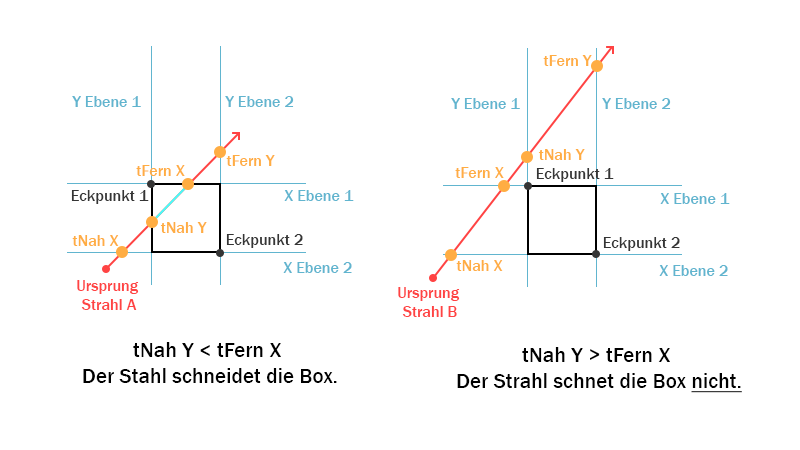
\includegraphics[width=0.9\linewidth]{images/rayBox.png}
	\caption{Zweidimensionale Darstellung, wie ein Strahl durch einen Würfel (links) und daran vorbei (rechts) verläuft. Die Schnittpunkte des Strahls (gelb) mit den Würfelebenen (blau) sind eingezeichnet. Der Vergleich derer Abstände zum Ursprung des Strahls (rot) zeigt, ob der Strahl den Würfel schneidet oder nicht.}
	\label{img:rayBoxHit}
	\source{Eigene Darstellung}
\end{figure}
\FloatBarrier

%----------------------------------------
Die beiden t-Werte werden als $t_{nah}$ und $t_{fern}$ gespeichert.
Mit dem Ursprung des Strahls und $t_{fern}$ werden Anfang, Ende und die Länge des Strahls berechnet. Mit Hilfe der Länge kann ermittelt werden um wie weit pro Iteration am Strahl entlang gegangen werden soll. Dadurch wird der Strahl nur bis zu seinem Austritt aus dem Würfel abgetastet. 

In einer for-Schleife wird jeder Strahl nun abgetastet. In jeder Iteration wird jeweils ein Punkt betrachtet. Der Punkt verschiebt sich entlang des Strahls um die zuvor berechnete Distanz.
Für jeden Punkt werden zuerst die Texturkoordinaten berechnet.
Für die Koordinaten werden dann die jeweiliges Isowerte aus der 3D-Textur gelesen, die zuvor mit den MRT-Bildern befüllt wurde.

%---------------SAMPLE VOLUME-------------
Hierbei werden lediglich die Texturkoordinaten als Indices für die Textur verwendet. 
Der Isowert ist dabei im Alphakanal der Textur gespeichert. Da es sich nicht um eine Farbe sondern nur einen Grauwert handelt, können die anderen Farbkanäle der Textur mit dem Gradienten des jeweiligen Pixels befüllt werden. Darauf wird im Abschnitt \ref{gradienten} genauer eingegangen.

Der Isowert wird außerdem noch mit der Intensität multipliziert, die der Nutzer beeinflussen kann.
An dieser Stelle wird aber auch geprüft, ob der betreffende Punkt überhaupt zu sehen ist oder aufgrund der verschiebbaren Schichten nicht sichtbar sein sollte. 
Dazu wird zuerst der aktuell betrachtete Punkt mit der Rotationsmatrix des Volumens multipliziert.
Der Punkt wird dann mit den von Nutzer eingestellten minimalen und maximalen X-, Y-, und Z-Werten der verschiebbaren Schicht verglichen, die den sichtbaren Bereich definieren. Das Ergebnis des Vergleichs wird dabei in einer Variable gespeichert. Ist der Punkt kleiner als das Minimum oder größer als das Maximum wird 0 gespeichert, ansonsten 1. 
Die beiden Werte werden anschließend mit dem Isowert multipliziert. Ist einer der Werte 0, ist auch der ermittelte Isowert 0, was im Alphakanal totale Transparenz bedeutet. 
Das Ergebnis dieser Berechnung wird zunächst jedem Farbkanal zugewiesen.
%-----------------------------------------

An dieser Stelle wird über die Transferfunktion der entsprechende Alphawert aus der zugehörigen Textur gelesen. Dazu wird der Isowert als Index verwendet. Die Funktionsweise und Implementierung der Transferfunktion wird in der Sektion \ref{transfer} beschrieben.
% Bezug Transferfunktion!
Die Transferfunktion wird nur abgerufen, wenn der Isowert nicht 0 ist, da sonst die Transparenz überschrieben würde.
% Tranferfunktion bei index 0 auf 0000 setzen??
Ist die Farbe bekannt, wir der betrachtete Voxel illuminiert. Dies ist in der Sektion \ref{illumination} beschrieben. 
Der Alphawert der so erhaltenen Farbe wird noch einmal halbiert, um die Darstellung semi-transparent erscheinen zu lassen.
% WARUM
Schließlich wird der erhaltene Farbwert mit den vorhergehenden verrechnet. Die Komposition erfolgt dabei von vorne nach hinten, da der Strahl in dieser Richtung abgetastet wird, nach der in Kapitel \ref{grundlagen} beschriebenen Formel.
% Referenz GPU Gems
Wenn diese Farbe einen zuvor definierten Schwellenwert überschreitet wird die Schleife abgebrochen. 
Die Farbe wird schließlich noch auf einen Wert zwischen 0 und 1 festgesetzt und mit der Farbe der Maske verrechnet, die auf dem selben Weg aber ohne die Verwendung einer Transfertextur bestimmt wurde.

\subsection{Transferfunktion}
\label{transfer}

Wie beschrieben, wird die Transfertextur im Shader ausgelesen. Vorher wird sie von dem Skript 3DUI/Scripts/CreateTransferColorTexture.cs erzeugt, welches beim Ausführen der Szene 3DUI/Scenes/Load3DTexture.unity ausgeführt wird.
Um eine Transfertextur zu erzeugen, werden zunächst zwei Key-Value-Listen definiert, in denen über Kontrollpunkte bestimmte Isowerte einem Farb- oder Opazitätwert zugewiesen werden. Mit Hilfe einer Schleife wird dann eine 2D-Textur mit den Dimensionen 256 und 1 erstellt. Dabei wird für jeden X-Wert der Textur geprüft, ob er größer oder gleich dem Isowert des betrachteten Kontrollpunktes ist. Ist dies der Fall, wird der Pixel der Textur mit dem entsprechenden Wert besetzt. Dies geschieht für alle Kontrollpunkte.
Die Textur wird dann als 2D-Textur abgespeichert. Da allein die Isowerte als Index für die Zuordnung verwendet werden, handelt es sich eigentlich um eine eindimensionale Transferfunktion. 
Allerdings werden von \textit{Unity} keine 1D-Texturen als Shader-Eigenschaften unterstützt. Da die Verwendung einer 2D-Textur aber keine Nachteile aufweist, wird stattdessen eine 2D-Textur verwendet, die eine einzige Y-Koordinate besitzt. 
Die Textur wird dann über das Material an den Shader übergeben. Wie im Abschnitt \ref{3dImplementierung} beschrieben, wird die Textur dann mit Hilfe eines Index ausgelesen.

Die Erstellung einer passenden Transfertextur ist allerdings, wie beschrieben, sehr schwierig und es konnte im Rahmen dieser Arbeit keine sinnvollen Kontrollpunkte zur Einfärbung des Volumens ermittelt werden. Aus diesem Grund wird nur der Alphawert der Transferfunktion verwendet. Auf diese Weise werden irrelevante Bildinformationen, wie Umgebungsrauschen und der Schädel ausgeblendet, wobei die Struktur des Hirninneren bestehen bleibt. 

\subsection{Beleuchtung}
\label{illumination}

Das Volumen wird mit mit dem Phong-Beleuchtungsmodell illuminiert, wodurch es mehr Plastizität erhält. Das Modell wurde bereits in Kapitel \ref{grundlagen} detailliert beschrieben. Deshalb wird an dieser Stelle nur auf die Umsetzung im Shader eingegangen.
% Referenz? warum nicht blinn?
Wie beschrieben setzt sich das Modell aus drei Komponenten zusammen: Der ambienten und der diffusen Beleuchtung, sowie der spiegelnden Reflexion. Die Komponenten werden zusammen addiert, wodurch die endgültige Farbe entsteht. 
Die Koeffizienten werden im Shader durch Farben repräsentiert. Der diffuse Koeffizient ist dabei der vorher aus der Transferfunktion gelesene Farbwert. Um diesen nicht durch die ambiente Beleuchtung zu verfälschen, wird er mit einem konstanten Faktor multipliziert, um eine abgedunkelte Farbe zu erhalten, die als ambienter Wert verwendet wird. Die Reflextion wird weiß dargestellt.
%Als Reflexionsexponent hat sich der Wert ?10? als am besten erwiesen.
Um die Reflexion berechnen zu können müssen außerdem der Lichtvektor und die Normale bekannt sein.
Wie bereits erläutert, wird der Gradient eines Voxels als Normale verwendet. 
Der Vektor zum Licht wird aus der in \textit{Unity} eingebauten Shader-Variable \_WorldSpaceLightPos0 ausgelesen.
%\todo{P Unterscheidung direktionales und Punktlicht?}

\subsection{Gradientenberechnung}
\label{gradienten}


Die Gradienten werden vor dem Start der Anwendung berechnet und zusammen mit den Isowerten in eine 3D-Textur geschrieben. Der Gradientenvektor wird dabei in den RGB-Kanälen gespeichert und der Isowert im Alpha-Kanal, da es sich nur um einen einzelnen Wert handelt. 

Die Berechnung der Gradienten erfolgt im selben Schritt, wie das Übertragen der Skalarwerte aus den Bilddaten in eine 3D-Textur.
Dafür werden alle Bilddateien in einem Dateiverzeichnis, auf das ein vorher definierter Pfad zeigt, ausgelesen und in ein Array übertragen, das der Größe der Bilder entspricht. Die dritte Dimension des Arrays wird durch die Anzahl der Bilder bestimmt. 

Entsprechend der in Kapitel \ref{grundlagen} beschriebenen Finite-Differenzen-Methode, werden durch eine Convolution die Gradienten für jeden Farbwert berechnet und ebenfalls in ein Array gespeichert.
Das Gradientenarray wird anschließend mit Hilfe eines Gauß-Filters mit einer Kernelgröße von 5 und $\sigma=5.5$ geglättet, bevor die Werte in eine 3D-Textur gespeichert werden. 

Diese wird im Asset-Verzeichnis 3DTextures des Projektes abgelegt. Sie werden in der Szene referenziert, um bei Bedarf an einen Shader übergeben zu werden, der den entsprechenden Datensatz darstellt. 

\section{\textit{HoloLens}-spezifische Implementierung}
\label{plattformen}

\subsection{\textit{HoloLens}-Demo}
Im Rahmen der Arbeit wurde neben der endgültigen Anwendung zuerst auch eine prototypische Demo-Anwendung entwickelt, die die \textit{HoloLens}-eigenen Gesten genutzt hat. Die Anwendung hat eine zweidimensionale Darstellung der MRT-Bilder als Hologramm in den Raum projiziert, welches der Nutzer durch \textit{HoloLens}-eigene Gesten manipulieren konnte. Dabei wurden alle vorhandenen Manipulierungsformen eines Hologramms abgedeckt, sowie das Scrollen durch die Bildschichten. Um die \textit{HoloLens}-Gesten zu Nutzen wurde das \textit{HoloToolkit} verwendet. 
Anhand dieser Demo sollte geprüft werden, ob die Interaktionsmöglichkeiten, die die \textit{HoloLens} bietet ausreichend sind, um einem Neurologen die effektive Untersuchung von MRT-Bildern zu ermöglichen.
Weiterhin konnten durch das Testen einer realen Anwendung die Erwartungen und Anforderungen eines Arztes an mARt noch weiter spezifiziert werden.  

Wie im Kapitel \ref{konzept} erläutert, haben sich die Gesten der \textit{HoloLens} zwar als ausreichend erwiesen, machten aber die Verwendung von weiteren Bedienelementen notwendig. Der Wechsel zwischen den Manipulationsarten wurde über ein ausklappbares Menü realisiert. Alle Manipulationen erfolgen über \textit{Air tap} und das Bewegen der Hand. Bei eingeklapptem Menü kann der Nutzer so durch die Darstellung scrollen. Aus den beschriebenen Gründen wurde für die endgültige Implementierung der Anwendung die \textit{Leap Motion} in das System integriert.
% Genauer auf Implementierung eingehen
Der Prototyp wurde in der Szene 2DUI\_HololensDemo/Scenes/HololensDemo.unity realisiert und eine Datei zur Bereitstellung für die \textit{HoloLens} sowie ein Video der Anwendung ist im Ergänzungsmaterial zu finden.
Die Demo ist in Abbildung \ref{img:prototyp} dargestellt.

\begin{figure}[!htb]
	\centering
	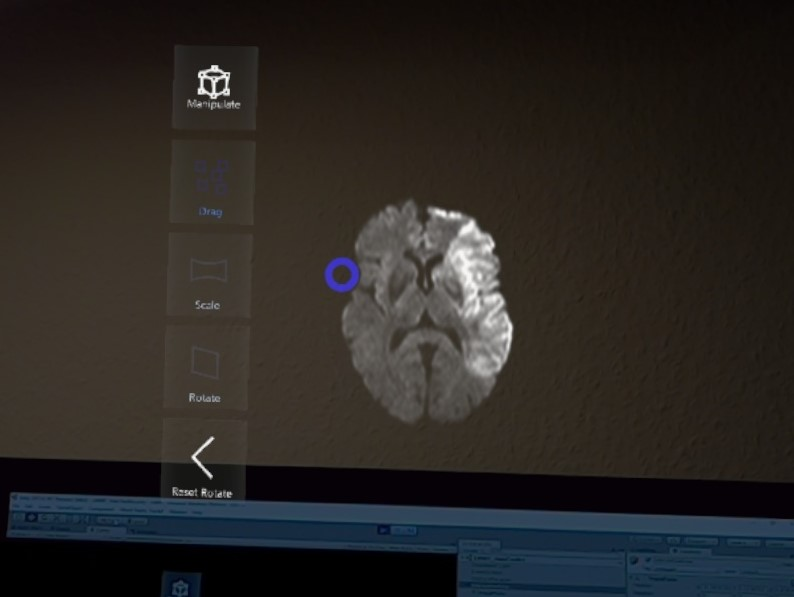
\includegraphics[width=0.5\linewidth]{images/hololens_prototyp.jpg}
	\caption{Aufnahme aus der \textit{HoloLens} von der \textit{HoloLens}-Demo, die Interaktionen ausschließlich über \textit{HoloLens}-Gesten realisiert.}
	\label{img:prototyp}
	\source{Eigene Darstellung}
\end{figure}
\FloatBarrier

\subsection{Positionierung im Raum}
\label{anchor}

Im Kapitel \ref{konzept} wurde bereits erwähnt, dass die dauerhafte Positionierung im Raum, wie sie \textbf{U17} fordert, auf unterschiedliche Weise implementiert werden kann. 
Die \textit{HoloLens} bietet diese Funktionalität in Form von Spatial oder World Anchors. Das Gerät besitzt einen internen Speicher für Anker, die von einer Anwendung angelegt werden, den sogenannten Anchor Store. Durch interne Prozesse bestimmt die \textit{HoloLens} in welchem Raum sie sich gerade befindet. Wird ein World Anchor in diesem Raum abgelegt, wird dessen Standort im Anchor Store gespeichert und behält somit immer seine Position im Raum, auch wenn der Nutzer sich bewegt und über mehrere Sitzungen hinweg. Nachdem ein World Anchor beim Start der Anwendung geladen wird, kann er an ein Objekt, wie ein 3D-Modell anhängt werden, sodass das Objekt an der Position des Ankers dargestellt wird. 

Ohne die Verwendung eines World Anchors wird die 3D-Szene und alle Objekte darin an der \textit{HoloLens} ausgerichtet, die den Nullpunkt der Szene darstellt. Durch die unterschiedliche Ausrichtung kommt es bei der Positionierung der Darstellung in der AR-Anwendung zu Komplikationen, sobald zwischen 2D- und 3D-Szene gewechselt wird. 

Der Anchor Store ist allerdings nur auf der \textit{HoloLens} verfügbar. Wie bereits erläutert wurde, wird die Anwendung im Rahmen dieser Arbeit aber nur auf der \textit{HoloLens} abgespielt, aber nicht für sie bereitgestellt. Dementsprechend ist ein Zugriff auf den Anchor Store nicht möglich. Dasselbe gilt für eine Verwendung der Anwendung in einem VR-System.

Als Alternative dazu können die Daten mit Hilfe eines Markers in den Raum projiziert werden, wie es im Kapitel \ref{grundlagen} beschreiben wurde. \textit{Unity} bietet hierfür das \textit{Vuforia}-Plugin, welches genau das umsetzt. Hierzu können Marker definiert werden, die das Programm erkennt und die diesen zugeordneten GameObjects anzeigt. 
\textit{Vuforia} ist für AR-Anwendungen gedacht und funktioniert durch eine Kamera, die den Marker erkennt. Deshalb kann die Funktion von einer \textit{Vive} nicht genutzt werden, von einer \textit{Vive Pro} jedoch schon, da diese über einen Mixed Reality Modus verfügt. Auch \textit{HoloLens}-Anwendungen können \textit{Vuforia} nutzen. 
Im zeitlichen Rahmen der Arbeit konnte dieses Funktionalität allerdings nicht mehr umgesetzt werden.

\section{Implementierung der Nutzereingabe}

\subsection{Verwendung der \textit{Leap Motion}}

Damit die \textit{Leap Motion} Kamera in einer Anwendung verwendet werden kann, muss das von \cite{orion} zur Verfügung gestellte SDK \textit{Orion} eingebunden werden. Das \textit{Core SDK} ist dabei zur Erkennung und Verwendung des Gerätes notwendig, während ein erweiterndes Paket Funktionen und Beispiele bietet, wie verschiedene Bedienelemente in eine Anwendung integriert werden können, die auf die Controller, also die Hände des Nutzers reagieren.
Meistens funktioniert dies indem einzelne Skripte, die das gewünschte Verhalten implementieren, als Components an GameObjects angehangen werden. Die Skripte lösen dann bestimmte Events oder Methoden aus, die mit den Funktionalitäten der Anwendung verknüpft werden. 

\subsection{Kombination von \textit{Leap Motion} mit \textit{Vive}/\textit{HoloLens}}
\label{kombination}

Sowohl \textit{Vive} als auch \textit{HoloLens} sollen in Verbindung mit der \textit{Leap Motion} funktionieren. Dazu muss zum Einen die \textit{Leap Motion} Kamera in beide Systeme integriert werden und zum Anderen die Funktionalität in die jeweiligen \textit{Unity} Szenen eingebaut werden. 

Das Einbinden der \textit{Leap Motion} in eine VR Anwendung, sowie die Kombination mit dem \textit{Vive} Headset sind unproblematisch. Das \textit{Orion} SDK der \textit{Leap Motion} unterstützt den Einsatz in VR-Szenen. Sofern \textit{SteamVR} installiert und eine VR-Brille angeschlossen ist, ist kein größerer Aufwand nötig, um die Hände des Nutzers in VR anzuzeigen. 
Die Integration in das VR-System ist vergleichbar einfach. Die \textit{Leap Motion} Kamera wird vorne auf dem HMD über der eingebauten Kamera befestigt und ihre Kabel zusammen mit den anderen der Brille über den Kopf des Nutzers geführt. 

Dagegen bringt die Verbindung von \textit{Leap Motion} und \textit{HoloLens} einige Herausforderungen mit sich. Zunächst ist in einer \textit{HoloLens}-Szene nur eine Kamera, die des HMDs, vorgesehen. Das Vorhandensein einer zweiten Kamera, wie die der \textit{Leap Motion} würde beim Erstellungsprozess zu Fehlern führen, sodass das Bereitstellen des Programmes für die \textit{HoloLens} nicht möglich ist.
Die \textit{Leap Motion} wird über ihr Kabel mit Strom versorgt. Sie kann also im Gegensatz zu der \textit{HoloLens} nicht kabellos funktionieren. 
Über das Kabel werden außerdem die von der \textit{Leap Motion} Kamera erfassten Daten weitergeleitet, die dann verarbeitet werden. Die dafür notwendige Software ist nicht für die \textit{HoloLens} verfügbar und es ist fragwürdig, ob sie die dafür notwendige Rechenleistung besitzt. 

Aus diesen Gründen muss die \textit{Leap Motion} während des Betriebs per Kabel mit einem Rechner verbunden sein. Um das Gerät trotzdem in Verbindung mit der \textit{HoloLens} nutzen zu können, müssen entweder die Sensordaten der \textit{Leap Motion} an die Anwendung in der \textit{HoloLens} übertragen werden oder die gesamte Anwendung läuft auf dem Rechner und wird zur Wiedergabe an die \textit{HoloLens} übermittelt. Beides geschieht über Wlan.

Die Übertragung der Sensordaten ist dabei um einiges aufwändiger und erfordert die Integration weiterer Tools. Es existieren einige Lösungsansätze für dieses Problem, beispielsweise von \cite{hololensGithub}. Auf Grund des beschränkten Zeitraums dieser Arbeit wurde dieser Ansatz allerdings nicht implementiert.
Stattdessen wird die Anwendung lediglich auf der \textit{HoloLens} wiedergegeben. Dazu wird die \textit{Hololens}-App \textit{Holographic Remoting Player} von \cite{remoteApp} genutzt. Die Anwendung wird dabei direkt aus dem \textit{Unity}-Editor übertragen.
Die Wiedergabequalität der Anwendung ist dabei abhängig von der Stabilität der Wlan-Verbindung.

Auch das Anbringen der \textit{Leap Motion} an das HMD ist bei der \textit{HoloLens} umständlicher als bei der \textit{Vive}. 
Da die \textit{Vive} einen undurchsichtigen Bildschirm besitzt, kann die \textit{Leap Motion} Kamera einfach vorne auf der Brille befestigt werden. Die Form des Gerätes bietet dazu ausreichend Fläche.
Bei der \textit{HoloLens} sollte der Bildschirm, durch den der Nutzer sieht nicht verdeckt werden. Eine Installation im oberen Teil der Frontseite ist ebenfalls nicht umsetzbar, da dieser von den \textit{HoloLens}-Kameras eingenommen wird, die die Umgebung und Nutzergesten verfolgen.
Somit ist die einzige sinnvolle Möglichkeit, die \textit{Leap Motion} auf der \textit{HoloLens} zu platzieren. Hierbei muss sie außerdem nach vorne geneigt werden, um die Hände des Nutzers in der Anwendung möglichst genau an den realen Händen auszurichten. 

% Ergebnisse


%\chapter{Ergebnisse}
\section{Ergebnisse}
\label{ergebnisse}

Die VR-Anwendung ist als ausführbare Datei im Ergänzungsmaterial zu finden. Da die \textit{HoloLens}-Anwendung, wie in Kapitel \ref{konzept} erläutert, nicht für diese bereitgestellt werden konnte, existiert hierfür keine ausführbare Datei. Allerdings wurde in der ReadMe.txt Datei des Projektes, welches sich ebenfalls im Ergänzungsmaterial befindet beschrieben, wie die Anwendung auf der \textit{HoloLens} abgespielt werden kann. 
Weiterhin ist dort ein Video enthalten, das die Funktionen und Bedienung der Anwendung zeigt.
Die Interaktionslemente wurden wie in Kapitel \ref{konzept} beschrieben implementiert. Neben ihrer Beschreibung sind dort auch Abbildungen der Benutzerelemente zu finden. 


\subsection{3D-Darstellung}

In Abschnitt \ref{3dImplementierung} wurde erläutert, wie die 3D-Darstellung mit Hilfe von Volume Raycasting erzeugt wurde. 
Dazu wurde der Alphawert einer Transfertextur genutzt, um das Rauschen in der Umgebung des Gehirns zu entfernen und die Gehirnform eindeutiger herauszustellen. Dies führt allerdings auch zu Artefakten, dem sogenannten Holzmaserungseffekt. Da allerdings die Darstellung der inneren Strukturen des Gehirns im Vordergrund steht, wurde sich für eine Darstellung entschieden, die durch Reduzierung der Umgebung den Fokus auf das Gehirn erlaubt. 
Im Abbildung \ref{img:resultsDWI} sind die beiden Datensätze mit und ohne die Verwendung einer Transferfunktion abgebildet. Durch Manipulation der Intensität kann bestimmt werden, in welcher Opazität das Gewebe gerendert werden soll, was vor allem das äußere Gewebe beeinflusst. Die Intensität der Renderings in der Abbildung ist in allen Fällen gleich.
Es ist anzumerken, dass die Qualität der Daten sich unweigerlich auf die Qualität des Renderings auswirkt. Die vorgegebenen Datensätze des Gehirns weisen ein hohes Maß an Bildrauschen auf. Außerdem wurden die Schichten offenbar in Abständen solcher Größe gescannt, dass die Interpolation zwischen den Schichten Aktefakte ausweist. Auch dies in in Abbildung \ref{img:resultsDWI} zu sehen.

\begin{figure}[!htb]
	\centering
	\includegraphics[width=0.9\linewidth]{images/dwi_results.png}
	\caption{Rendering der zur Verfügung gestellten Datensätze durch den in mARt verwendeten Shader mit gleicher Intensität. a) Datensatz 1 ohne Transferfunktion b) Datensatz 1 mit Transferfunktion c) Datensatz 2 ohne Transferfunktion d) Datensatz 2 mit Transferfunktion}
	\label{img:resultsDWI}
	\source{Eigene Darstellung}
\end{figure}
\FloatBarrier
  
Aus diesem Grund wurden testweise auch andere Daten mit dem selben Shader gerendert. Das Ergebnis ist dabei von besserer Qualität als mit den Gehirndaten. Die Verwendung der Transferfunktion ist nicht notwendig, um die Darstellung deutlicher zu machen. In Abbildung \ref{img:resultsVisMale} ist der Datensatz eines Kopfes mit und ohne Transferfunktion dargestellt.
  
\begin{figure}[!htb]
	\centering
	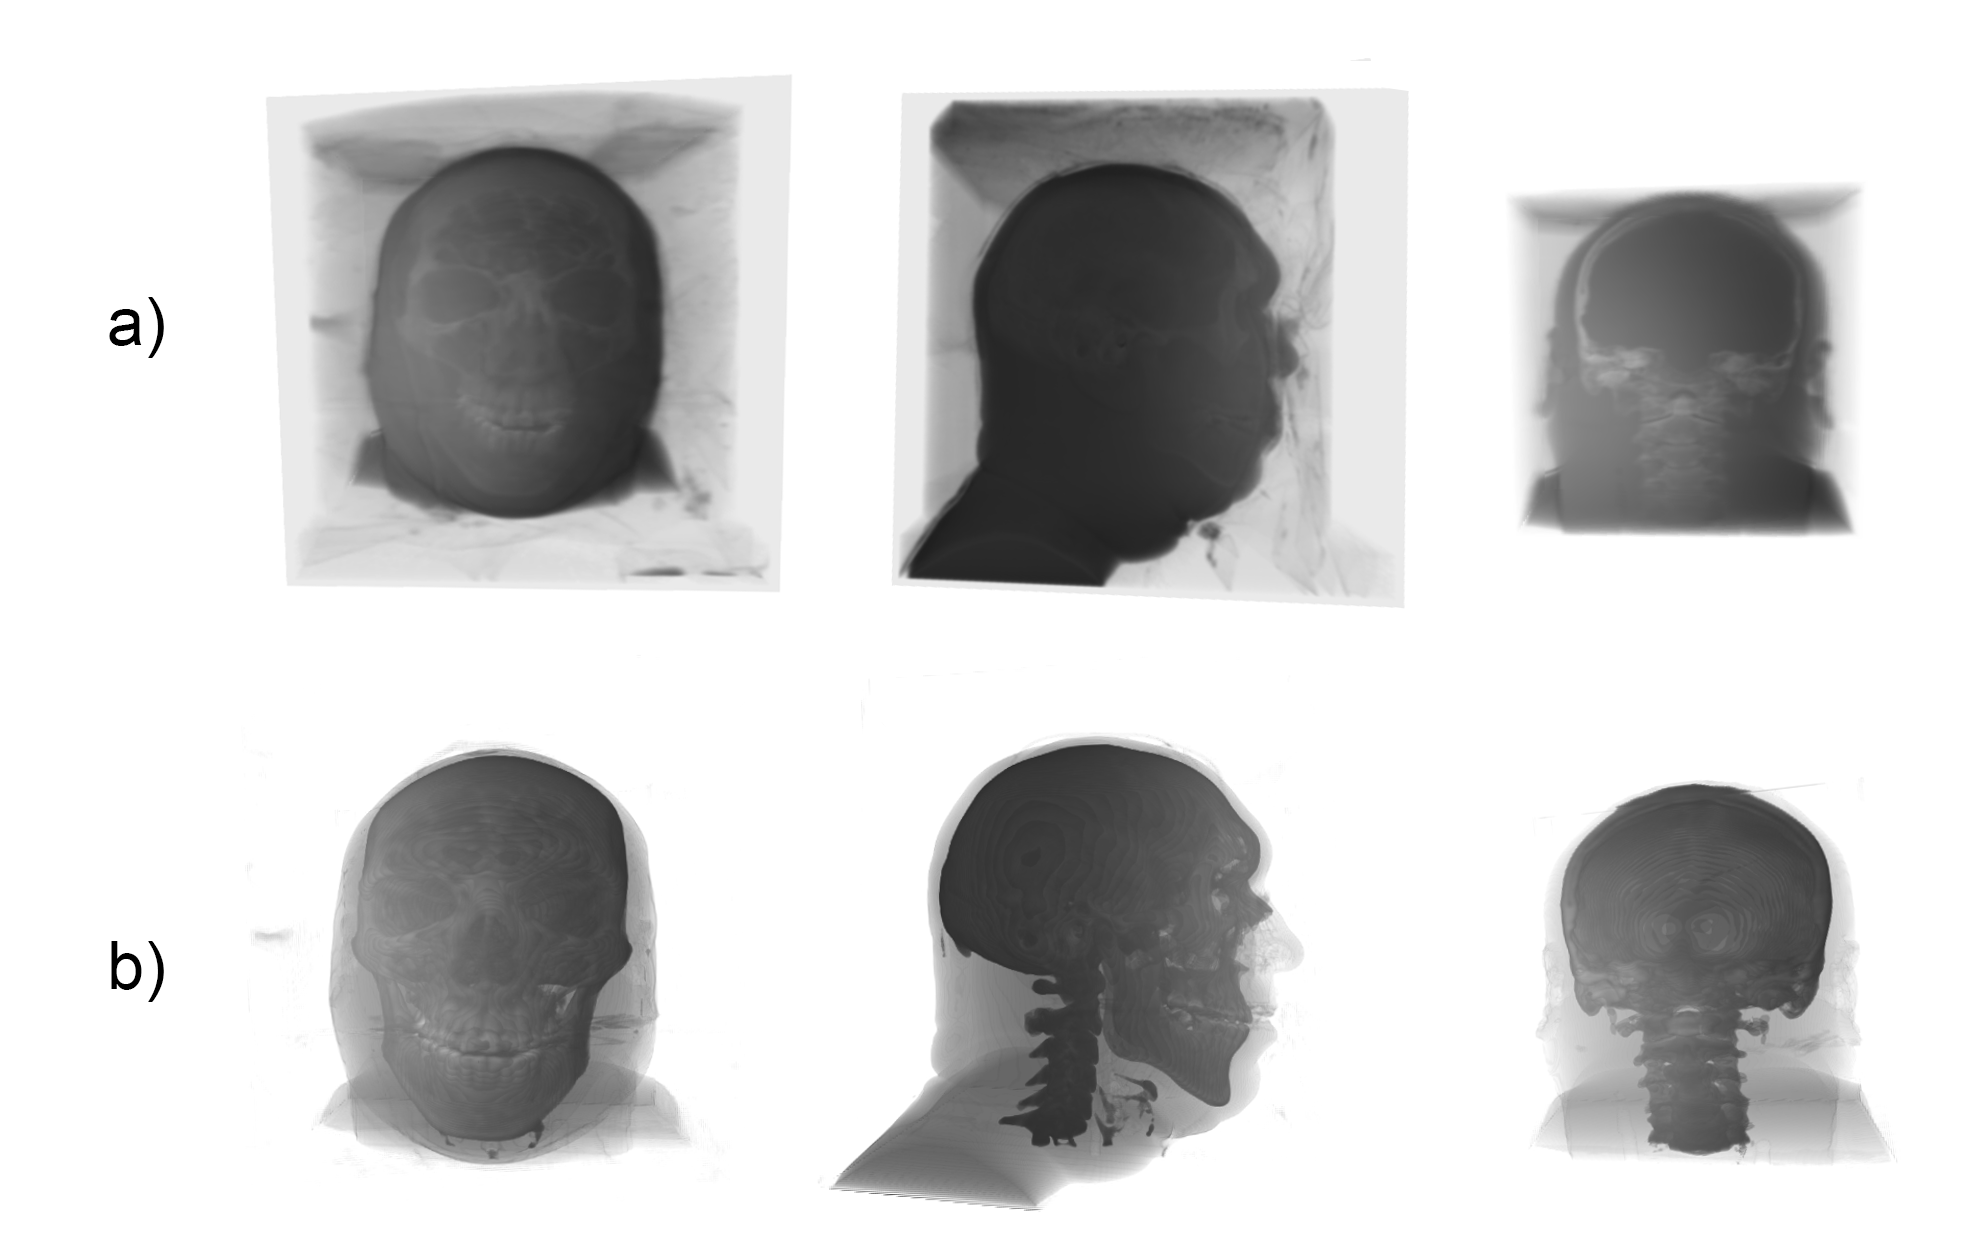
\includegraphics[width=0.9\linewidth]{images/visMale_result.png}
	\caption{Rendering eines alternativen Datensatzes durch den in mARt verwendeten Shader mit gleicher Intensität. a) Rendering ohne Transferfunktion b) Rendering mit Transferfunktion}
	\label{img:resultsVisMale}
	\source{Eigene Darstellung}
\end{figure}
\FloatBarrier

Der gekennzeichnete Bereich, der verdeutlicht welche Teile des Gehirns von dem Schlaganfall betroffen wurden, ist durch die semitransparente Darstellung von allen Seiten gut zu erkennen. 
Durch die Multiplikation der Masken- und Isowerte ist die Struktur des Gehirns weiterhin erkennbar. In Abbildung \ref{img:resultMask} sind Renderings des Gehirns und des Bereichs dargestellt.

\begin{figure}[!htb]
	\centering
	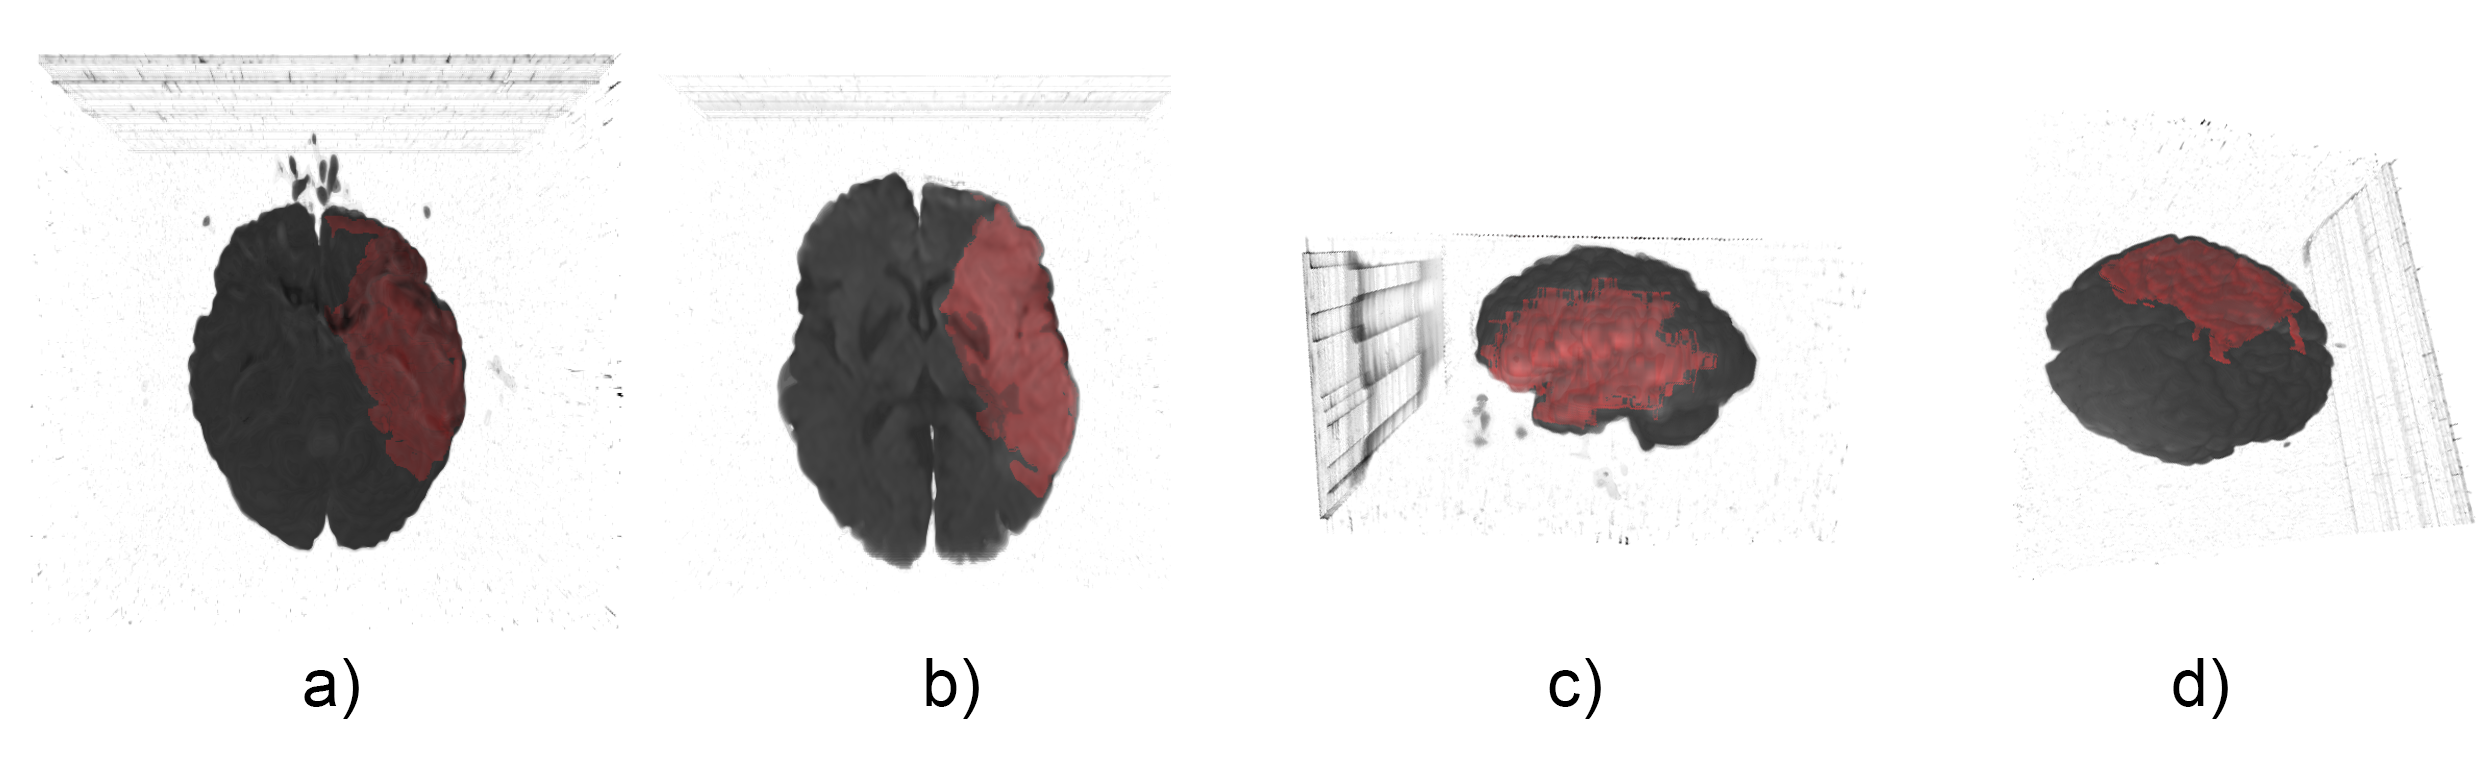
\includegraphics[width=0.99\linewidth]{images/mask_results.png}
	\caption{Rendering des ersten Datensatzes und der Maske, die den betroffenen Bereich hervorhebt, aus verschiedenen Ansichten.}
	\label{img:resultMask}
	\source{Eigene Darstellung}
\end{figure}
\FloatBarrier
  
\subsection{AR Anwendung}
Durch die semi-transparente Darstellung in AR sind die eher dunklen MRT-Daten teilweise schlecht zu erkennen. Dies betrifft vor allem die 3D-Darstellung. Um das Rendering erkennen zu können müssen die Farbwerte durch die Gammakorrektur erhellt werden. In Abbildungen \ref{img:ARLicht} und \ref{img:ARLicht3D} dargestellt, wie die Daten mit dem Standardhelligkeitswert und mit einem erhöhten Wert aussehen.

\begin{figure}[!htb]
	\centering
	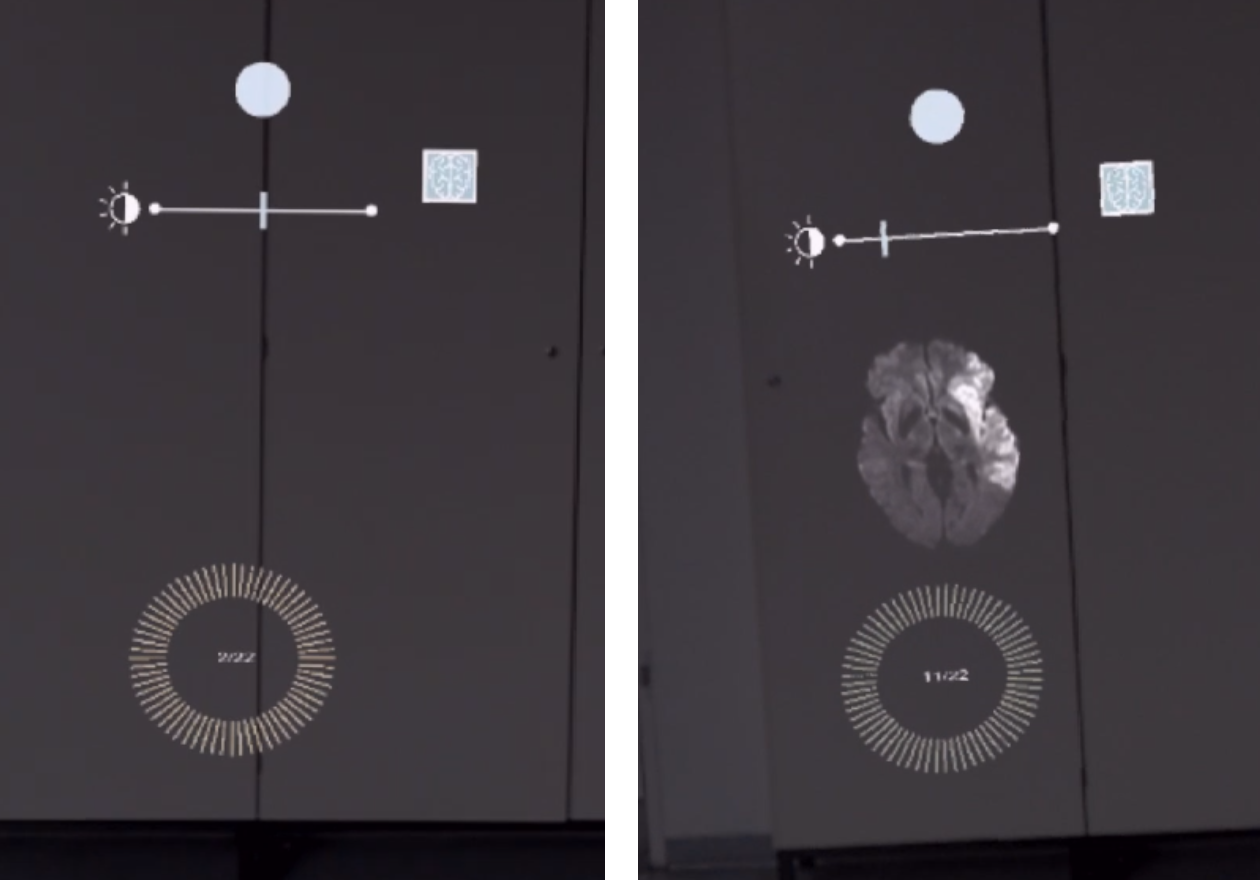
\includegraphics[width=0.7\linewidth]{images/mARt_AR_brightness.png}
	\caption{Zwei Aufnahmen aus der \textit{HoloLens}, während der 2D-Scene von mARt mit unverändertem (links) und erhöhtem (rechts) Gammakorrekturwert. Um die Darstellung erkennen zu können muss der Wert erhöht werden.}
	\label{img:ARLicht}
	\source{Eigene Darstellung}
\end{figure}
\FloatBarrier

\begin{figure}[!htb]
	\centering
	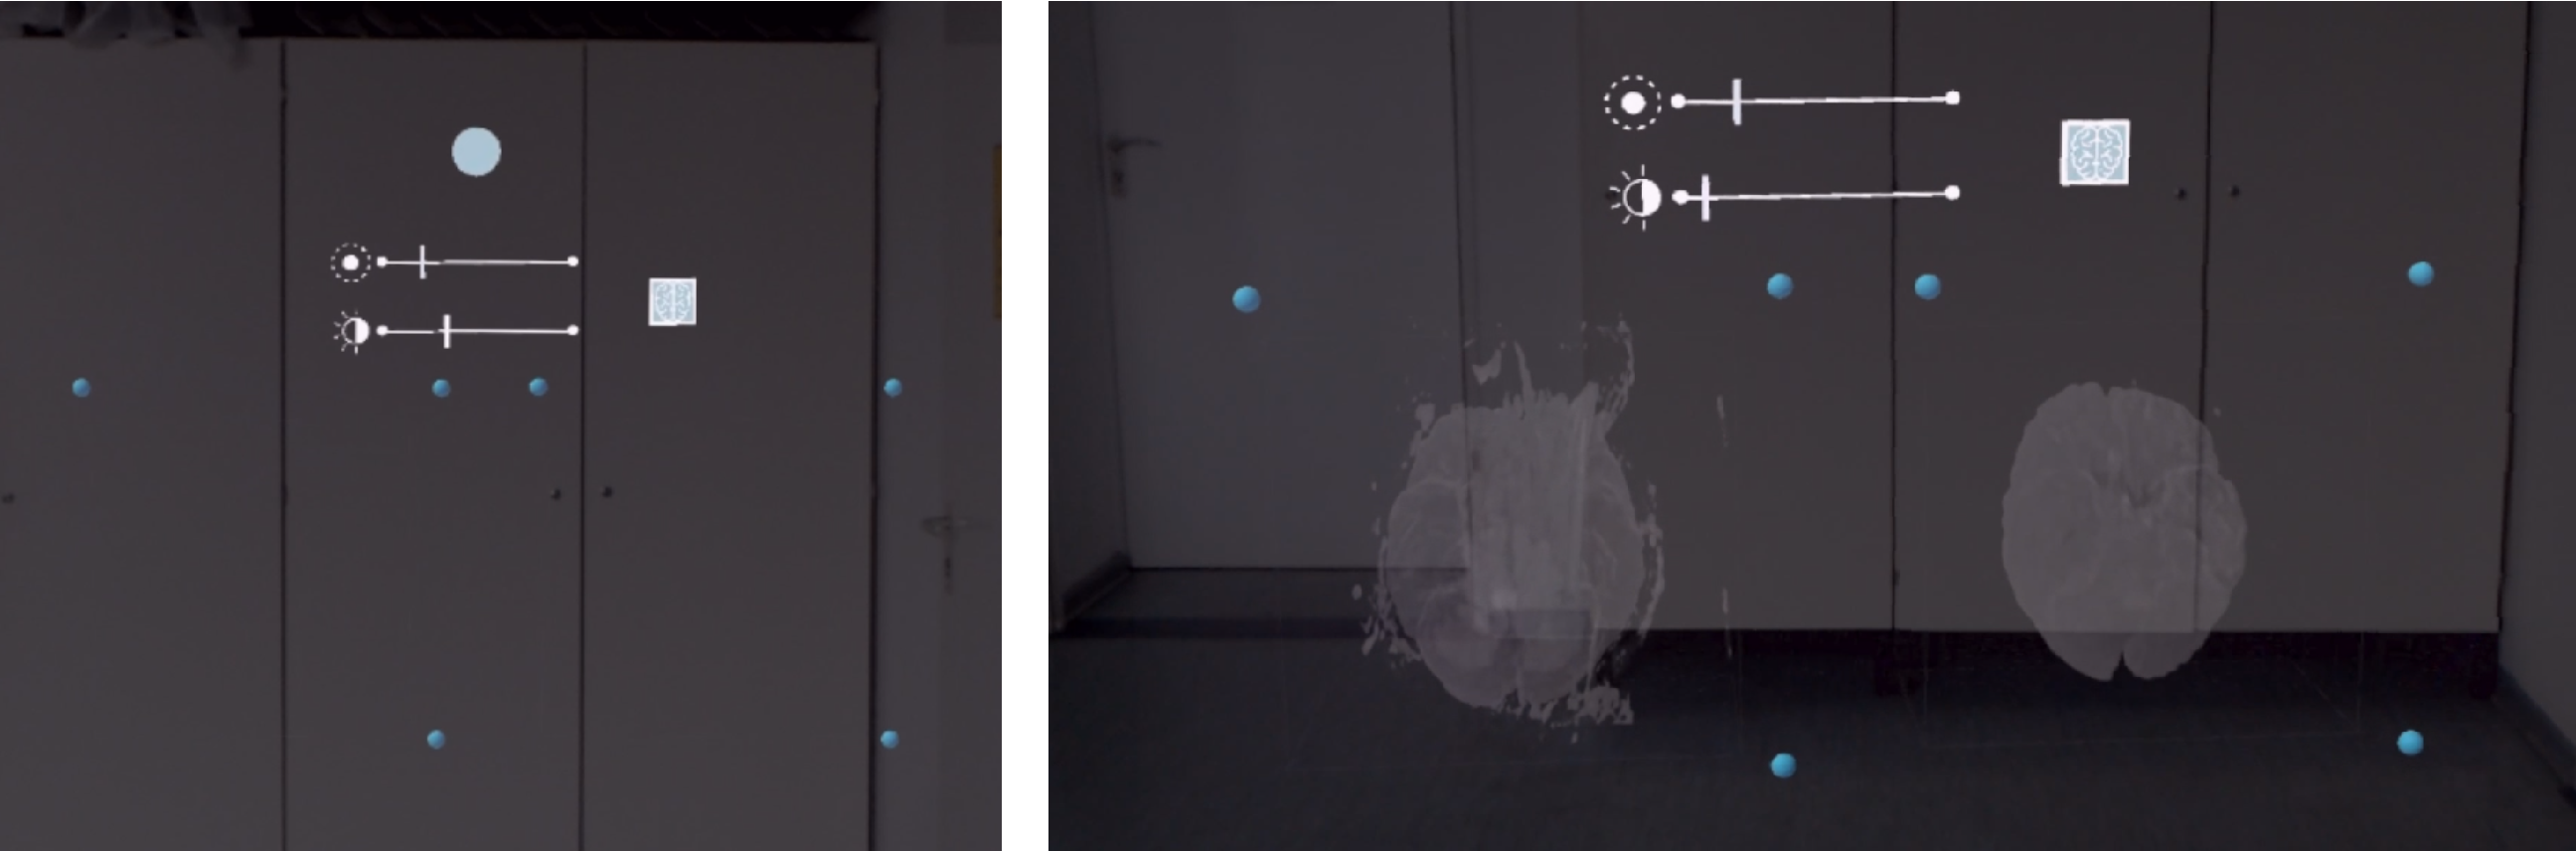
\includegraphics[width=0.9\linewidth]{images/mARt_AR_brightness_3D.png}
	\caption{Zwei Aufnahmen aus der \textit{HoloLens}, während der 3D-Scene von mARt mit unverändertem (links) und erhöhtem (rechts) Gammakorrekturwert. Um die Darstellung erkennen zu können muss der Wert erhöht werden.}
	\label{img:ARLicht3D}
	\source{Eigene Darstellung}
\end{figure}
\FloatBarrier

Ein weiterer Punkt, der die Verwendung der Anwendung auf der \textit{HoloLens} erschwert, ist das eingeschränkte Sichtfeld des Gerätes. Dieses Problem wurde bereit in Kapitel \ref{grundlagen} beschrieben. 
Die Begrenzung der Darstellung führt dazu, dass die MRT-Daten aus der Sicht des Nutzers meist abgeschnitten sind. Um die Daten gleichzeitig mit den Interaktionselementen sehen zu können, muss der Nutzer einen Abstand von ca. 1,5m zur Darstellung haben. Dies macht es ihm allerdings unmöglich mit dieser zu interagieren. Um die Darstellung manipulieren zu können, muss er also zwischen MRT-Bildern und Bedienelementen hin- und herblicken. In Abbildung \ref{img:ARCutoff} ist das abgeschnittene Sichtfeld der \textit{HoloLens} dargestellt. Dabei werden die virtuellen Hände des Nutzer nicht angezeigt, wenn er diese nicht direkt ansieht, auch wenn die Leap Motion diese vielleicht noch erfasst. 
Die Darstellung der Hände selbst nimmt bereits einen großen Teil des Sichtfeldes der \textit{HoloLens} ein, da sie sich nah am HMD befinden. 
Eine Bedienung der Anwendung auf der \textit{HoloLens} ist aus diesen Gründen sehr schwer. 

\begin{figure}[!htb]
	\centering
	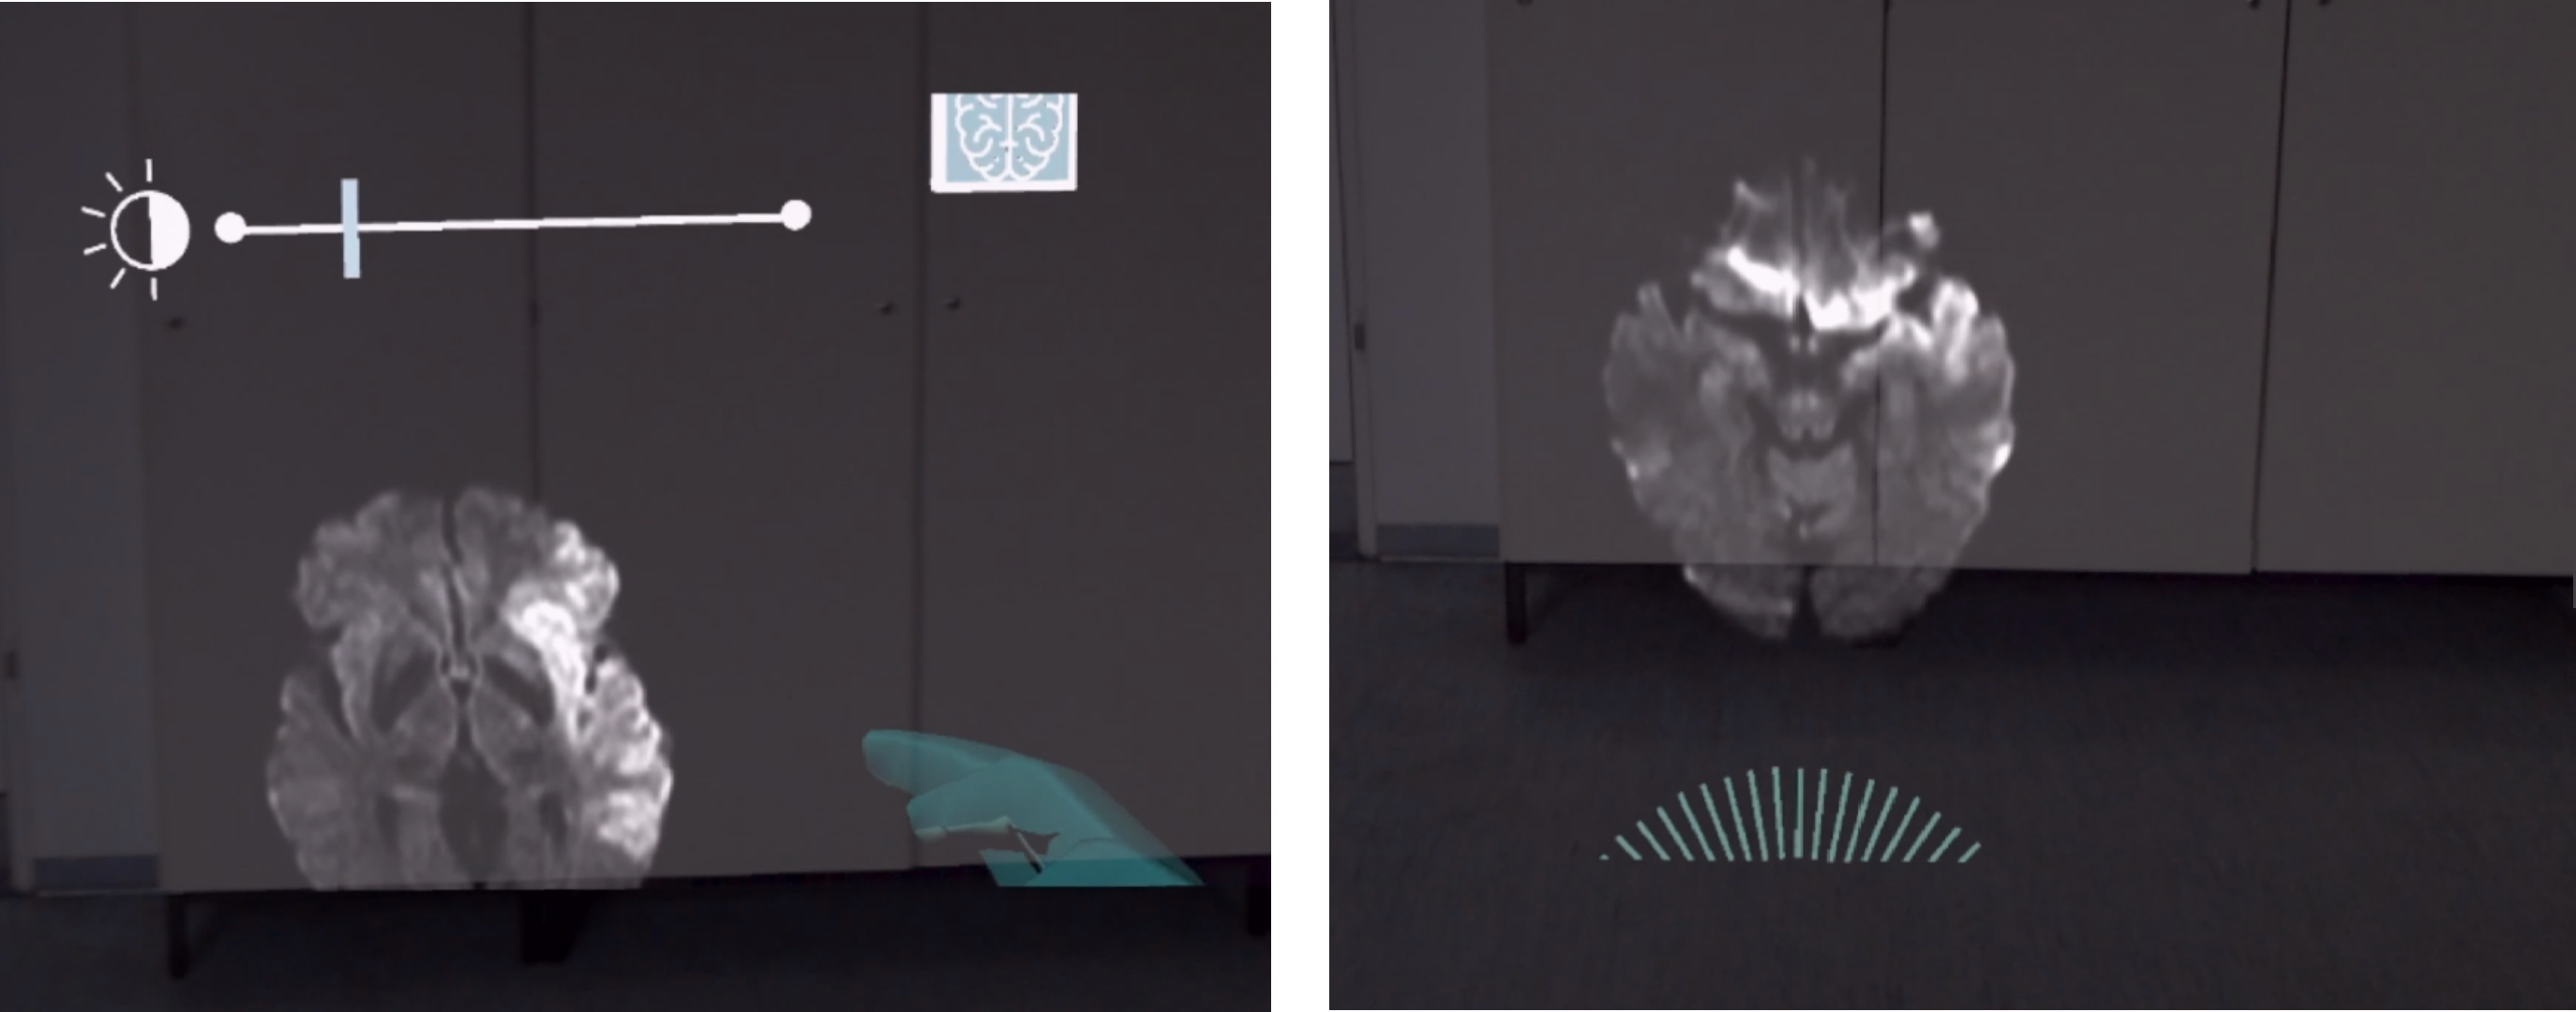
\includegraphics[width=0.9\linewidth]{images/mARt_Cutoff.png}
	\caption{Zwei Aufnahmen aus der \textit{HoloLens}, während der 2D-Scene von mARt aus bedienbarer Entfernung. Durch das begrenzte Sichtfeld der \textit{HoloLens} wir nur ein Ausschnitt der Anwendung dargestellt.}
	\label{img:ARCutoff}
	\source{Eigene Darstellung}
\end{figure}
\FloatBarrier

